%
% File acl2021.tex
%
%% Based on the style files for EMNLP 2020, which were
%% Based on the style files for ACL 2020, which were
%% Based on the style files for ACL 2018, NAACL 2018/19, which were
%% Based on the style files for ACL-2015, with some improvements
%%  taken from the NAACL-2016 style
%% Based on the style files for ACL-2014, which were, in turn,
%% based on ACL-2013, ACL-2012, ACL-2011, ACL-2010, ACL-IJCNLP-2009,
%% EACL-2009, IJCNLP-2008...
%% Based on the style files for EACL 2006 by 
%%e.agirre@ehu.es or Sergi.Balari@uab.es
%% and that of ACL 08 by Joakim Nivre and Noah Smith

\documentclass[11pt,a4paper]{article}
\usepackage[hyperref]{acl2021}
\usepackage{times}
\usepackage{latexsym}
\usepackage{graphicx}
\usepackage{minted}
\renewcommand{\UrlFont}{\ttfamily\small}

% This is not strictly necessary, and may be commented out,
% but it will improve the layout of the manuscript,
% and will typically save some space.
\usepackage{microtype}

\aclfinalcopy
%\def\aclpaperid{***} %  Enter the acl Paper ID here

%\setlength\titlebox{5cm}
% You can expand the titlebox if you need extra space
% to show all the authors. Please do not make the titlebox
% smaller than 5cm (the original size); we will check this
% in the camera-ready version and ask you to change it back.

% Content lightly modified from original work by Jesse Dodge and Noah Smith


\newcommand\BibTeX{B\textsc{ib}\TeX}

\title{Reproducibility Project of Density-Aware Personalized Training for Risk Prediction in Imbalanced Medical Data}

\author{Kaley Nguyen \\
  \texttt{\{kaleynn2\}@illinois.edu}
  \\[2em]
  Group ID: 103\\
  Paper ID: 81 "Density-Aware Personalized Training for Risk Prediction in Imbalanced Medical Data" \cite{huo2022densityaware}\\
  Presentation link: \url{https://www.youtube.com/working_on_it} \\
  Code link: \url{https://github.com/kaleynguyen/cs598-dlh/tree/main/project}} 


\begin{document}
\maketitle

% All sections are mandatory.
% Keep in mind that your page limit is 8, excluding references.
% For specific grading rubrics, please see the project instruction.

\section{Introduction}
Since public health data follow a long tail distribution \cite{longtail}, many medical events are rare events. In the past, researchers have attempted to solve the issue by either undersampling the majority class, oversampling the minority class \cite{sampling} or use synthetic examples to account for imbalance \cite{smote}. The authors of the article suggest the following framework for training the data with the imbalance problem: 1. Separate the feature extraction and classification processes; 2. Train the network using a loss function that takes into account density and a learnable cost matrix for misclassifications. Using the real-world medical datasets (MIMIC-III), the model's performance metrics for imbalanced class are improved, as evidenced by the AUC-ROC, AUC-PRC, and Brier Skill Score.

\section{Scope of reproducibility}

The paper introduces a new approach to handle imbalanced medical data set by exploiting the imbalanced densities and training the network with a density-aware hinge loss function to improve the performance metric by 4.7\% (max percent change AUC-ROC) and 14.2\% percent (max percent change AUC-PRC) compared to the baselines of mortality prediction on MIMIC-III dataset. 

The paper does not provide the source code to reproduce the result. However, the paper links the architecture of the deep learning model \cite{deasy2019impact} at \url{https://github.com/jacobdeasy/flexible-ehr}. Each of the step below corresponds to the scripts at ```flexehr/scripts/[1-7].py```.

\begin{enumerate}
    \item Separate patients as described in the MIMIC-III benchmark \cite{mimiciiibenchmark} as below with mortality prediction task. 
    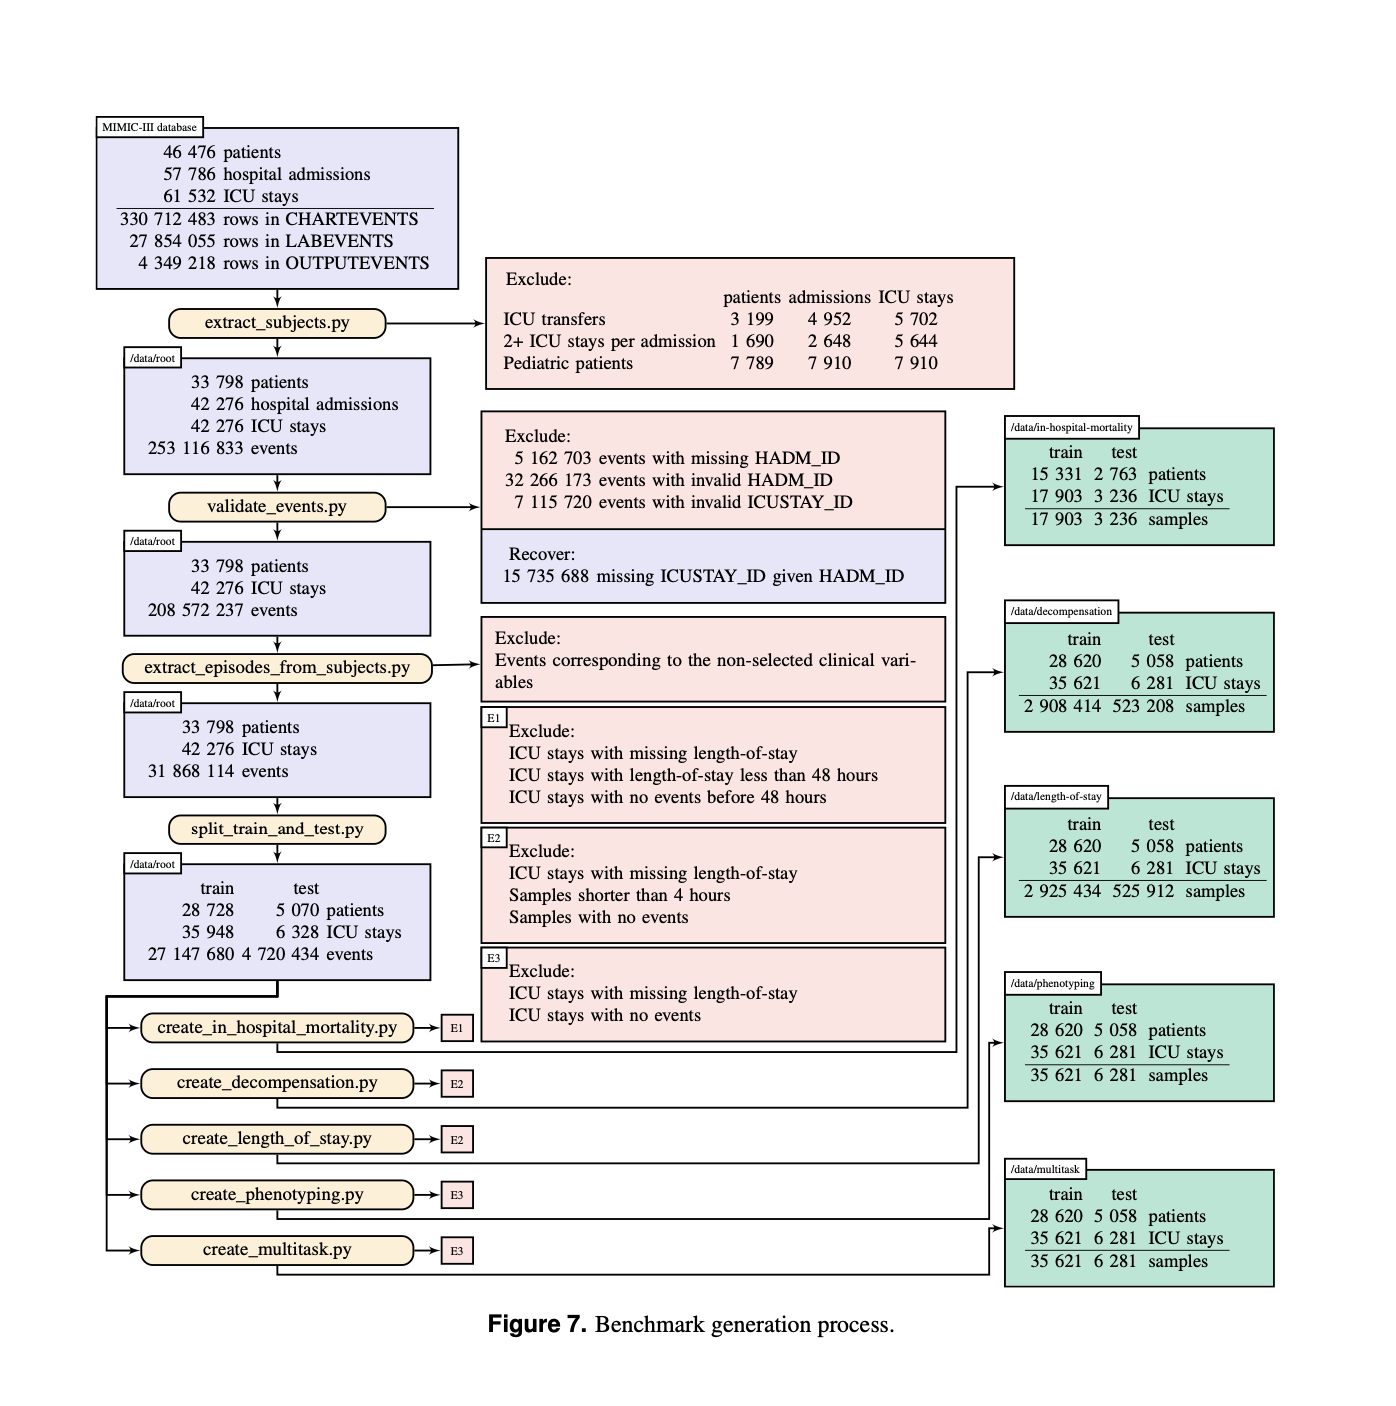
\includegraphics[scale=0.35]{acl-ijcnlp2021-templates/image/dataprocess.png}
    \item Extract individual stays from each patient. Patient data is simply separated by admission information.
    \item Truncate times series to t hours and store in data/root.
    \item Split the data into training, validation and test set.
    \item Generate a dictionary of labels to value arrays from ITEMIDs and values.
    \item Quantize events into n bins based on dictionary labels to values.
    \item Create final arrays for training.
\end{enumerate}



\subsection{Predictive Power and Performance Metrics}
The authors propose a framework for addressing class imbalance density (7-10\%) and utilizing the imbalance to provide density-aware training for enhanced risk prediction performance.  

The framework proposes some ideas: 
\begin{itemize}
    \item The risk prediction performance can be improved by decoupling the training of representation learning and classification to extract class-specific features and predictions.  
    \item Differences in density are some features that should be learned, rather than attempted to be eliminated. 
    \item AUC-ROC is too confident to use as the only performance metric to address the rare medical event predictive power. 
\end{itemize}

\subsection{Discriminative Power}
The authors propose that  the patients who survived would be more similar to each other compared to the patients who did not survive. The embedded vector from the flexehr, which has 256-dimensions in the last hidden layer, is visualized into 2-dimensional tSNE \cite{tsne}.

\section{Methodology}

\begin{enumerate}
    \item Sampling 2 batches of data using 2 different sampling strategies, regular random sampling and stratified random sampling with class-balance probability. Both batches are used to  extract the embedding vectors with flexehr while the classifier only trains on the balanced batches.  
    \item The density-aware outlier detection loss replaces the log loss or cross entropy loss to address the imbalance issue. The density aware loss is similar to the hinge loss with a density aware component $\bigtriangleup_c$.
    \item Trainable cost matrix or confusion matrix is used to reduce the bias between the big class and small class by manipulating the type I (unnecessary medical intervention) and type II (misdiagnosis) error.   
\end{enumerate}

\subsection{Data descriptions}
For predicting a patient's mortality and phenotype, the authors only look at the first 48 hours after they are admitted to the ICU. The idea is that the precaution treatment can be done for early risk prognosis and phenotyping since the average stay in the ICU is 100 to 200 hours. The paper uses the same data pre-processing steps as a set of standard models in MIMIC-III \cite{mimiciiibenchmark} to build 34 time-series features using the same 17 clinical measurements. 

\subsection{Model descriptions}
\begin{itemize}
    \item Split the data using 80/10/10 splits. Use each data set to generate its respective class-balanced data set. 
    \item Train the model on flexehr, which is a GRU based method architecture with 50 epochs, batch size is 128 and the Adam optimizer with learning rate of 0.001 is used.
    \item AUC-ROC, AUC-PRC and BSS are used to measure the difficulty of discriminating power. 
    \item softmax is used in the last layer of the flexehr to obtain the predicted probability for the calibration study.  
\end{itemize}


\subsection{Hyperparameters}
\begin{itemize}
\item Density-aware component $\bigtriangleup_c = \frac{K}{|N_c|^{1/4}}$ for $c \in \{1,...,|C|\}$
where $K$ is a hyper-parameter and $|N_c|$ is number of examples in class $c$.

\item Relax the constrained problem as an unconstrained one and rewrite $C_{FN}$ = $\theta$ $C_{FP} + D $ to $C_{FP} > 0$  and change the loss function in terms of log$C_{FP}$ where D is a regularization term, $\theta$ is a hyper-parameter, $C_{FP}$ is a type I error, and $C_{FN}$ is a type II error in the confusion matrix. Notice that the trainable confusion matrix is only applicable for a binary classification problem. 
\end{itemize}

\subsection{Ablation Study}
In the paper, two new components are introduced: decoupling the training and a loss function that takes into account the density of the data. The paper suggests using the same architecture - flexEHR or GRU. Specifically, one GRU as a baseline, one GRU with the trainable cost matrix, one GRU with the decoupling method, and one GRU with both the decoupling method and the trainable cost matrix. In the ablation study, the AUC-ROC does not change significantly, but the AUC-PRC and BSS improve significantly. However, GRU-decoupling has poor calibrated range compared to the combined framework.  

\subsection{Implementation}
 \begin{enumerate}
     \item Access csv data from an S3 bucket at s3://mimic-iii-physionet. 
     \item Process data, follow the model descriptions to split the data, implement the custom loss function and train the model on a g5.4xlarge instance within the same availability zone in AWS (us-east-1). Save the model as pickle models 
     \item Test the models on the test set and compare the AUC-ROC, AUC-PRC and BSS between these models. 
     \item Visualize the density plot of survived/expired patients on the embedding vectors using t-SNE. 
     \item Plot the calibration to compare the calibrated ability between each of the model in the ablation study.  
 \end{enumerate}

\subsection{Computational requirements}
I plan to use the g5.4xlarge to process and run the model but my availability zone is different than the MIMIC-III's availability zone. I requested to get an additional ec2 g5.4xlarge instance on AWS. AWS declined. Currently, I used an iMac Apple M1 16GB memory on Ventura to run the pre-processing files on \url{https://github.com/jacobdeasy/flexible-ehr}. 

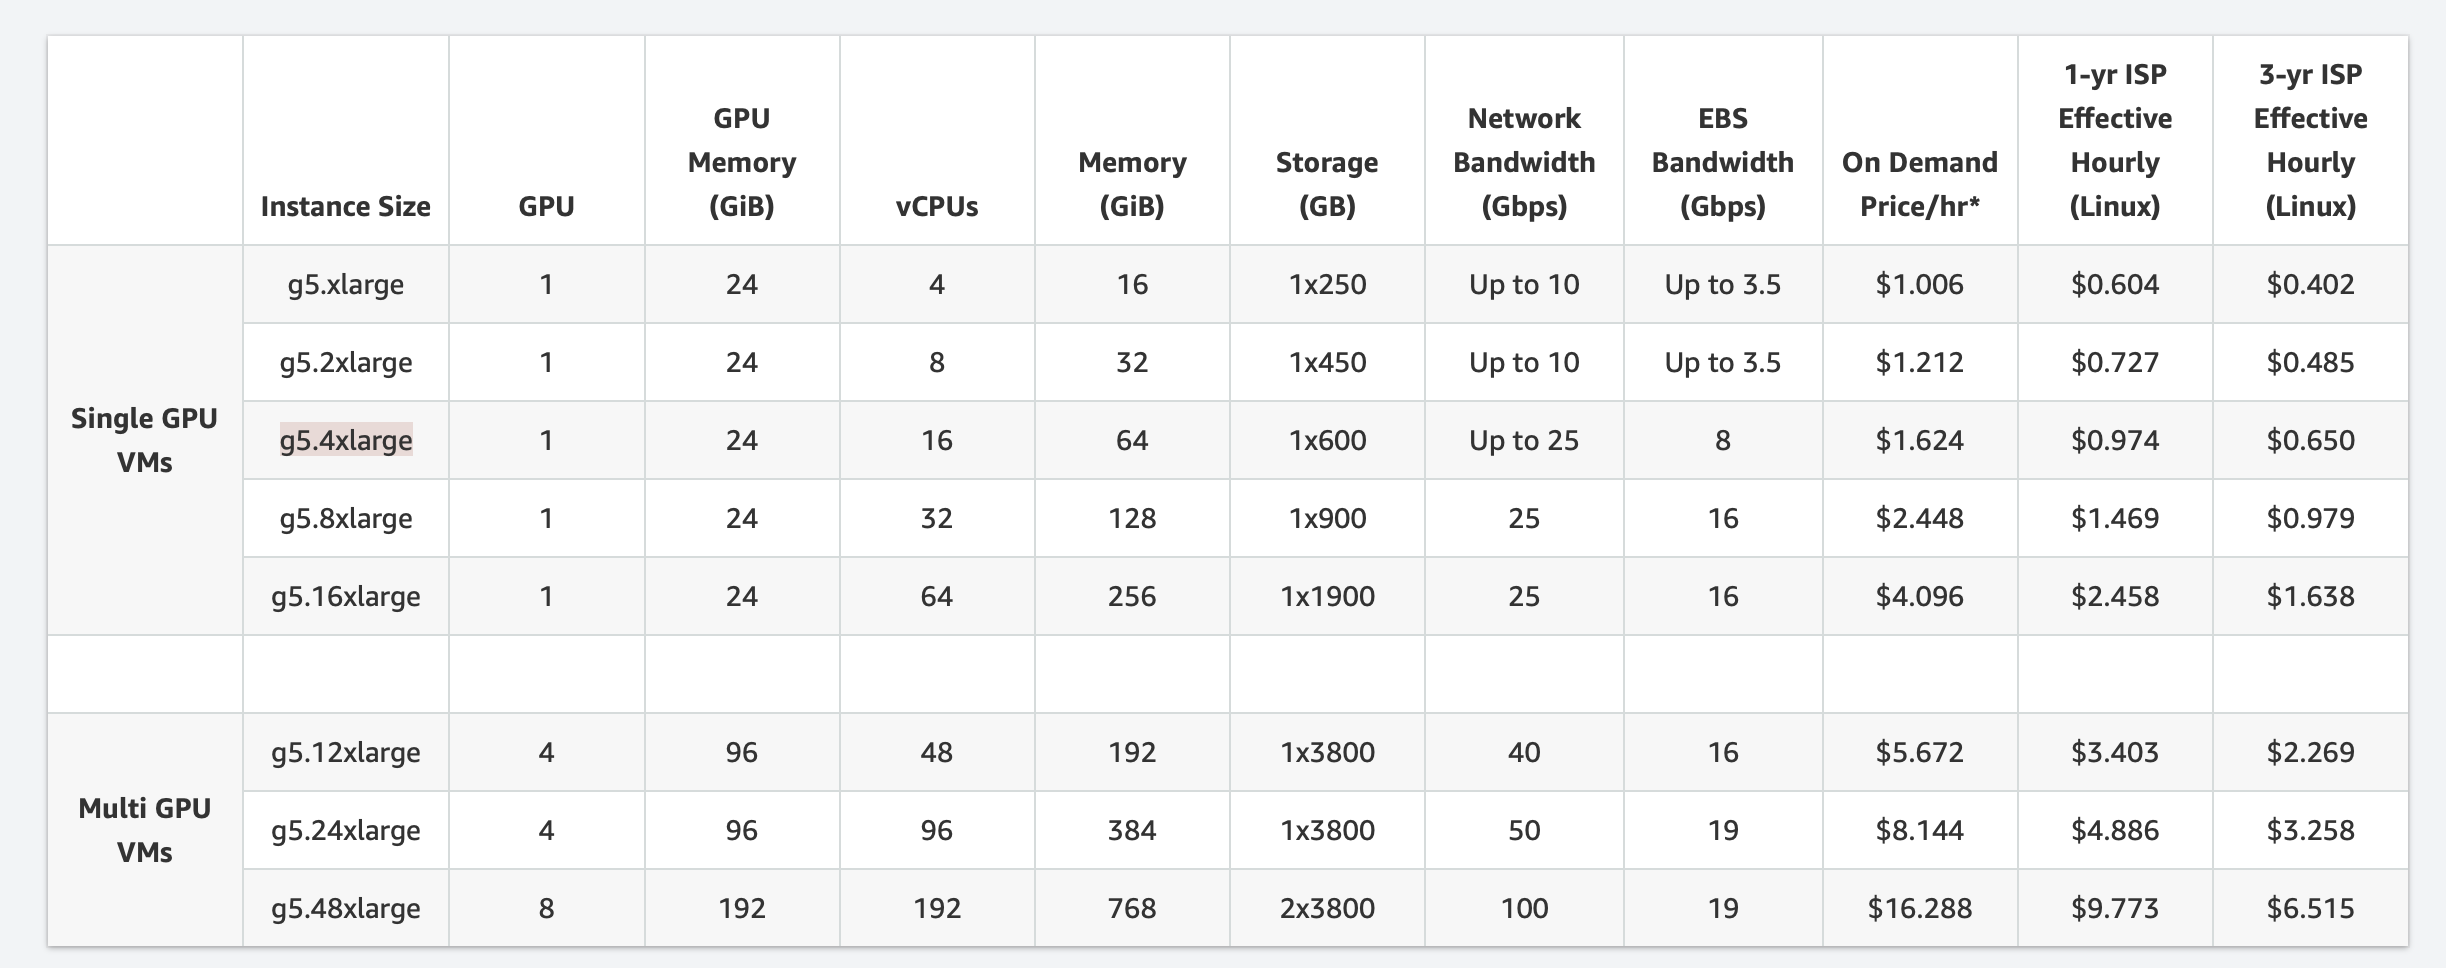
\includegraphics[scale=0.16]{acl-ijcnlp2021-templates/image/gpu.png}

\section{Results}

% The number of subsections for results should be the same as the number of hypotheses you are trying to verify.

\subsection{Result 1}
It took more than 7 hours to process the MIMIC-III data on the instance, so I am going to capture a screenshot of the process. I plan to re-write the pre-processing code in Polars on parquet files so it takes a significant less time than the current implementation of cleaning csv files in pandas. 

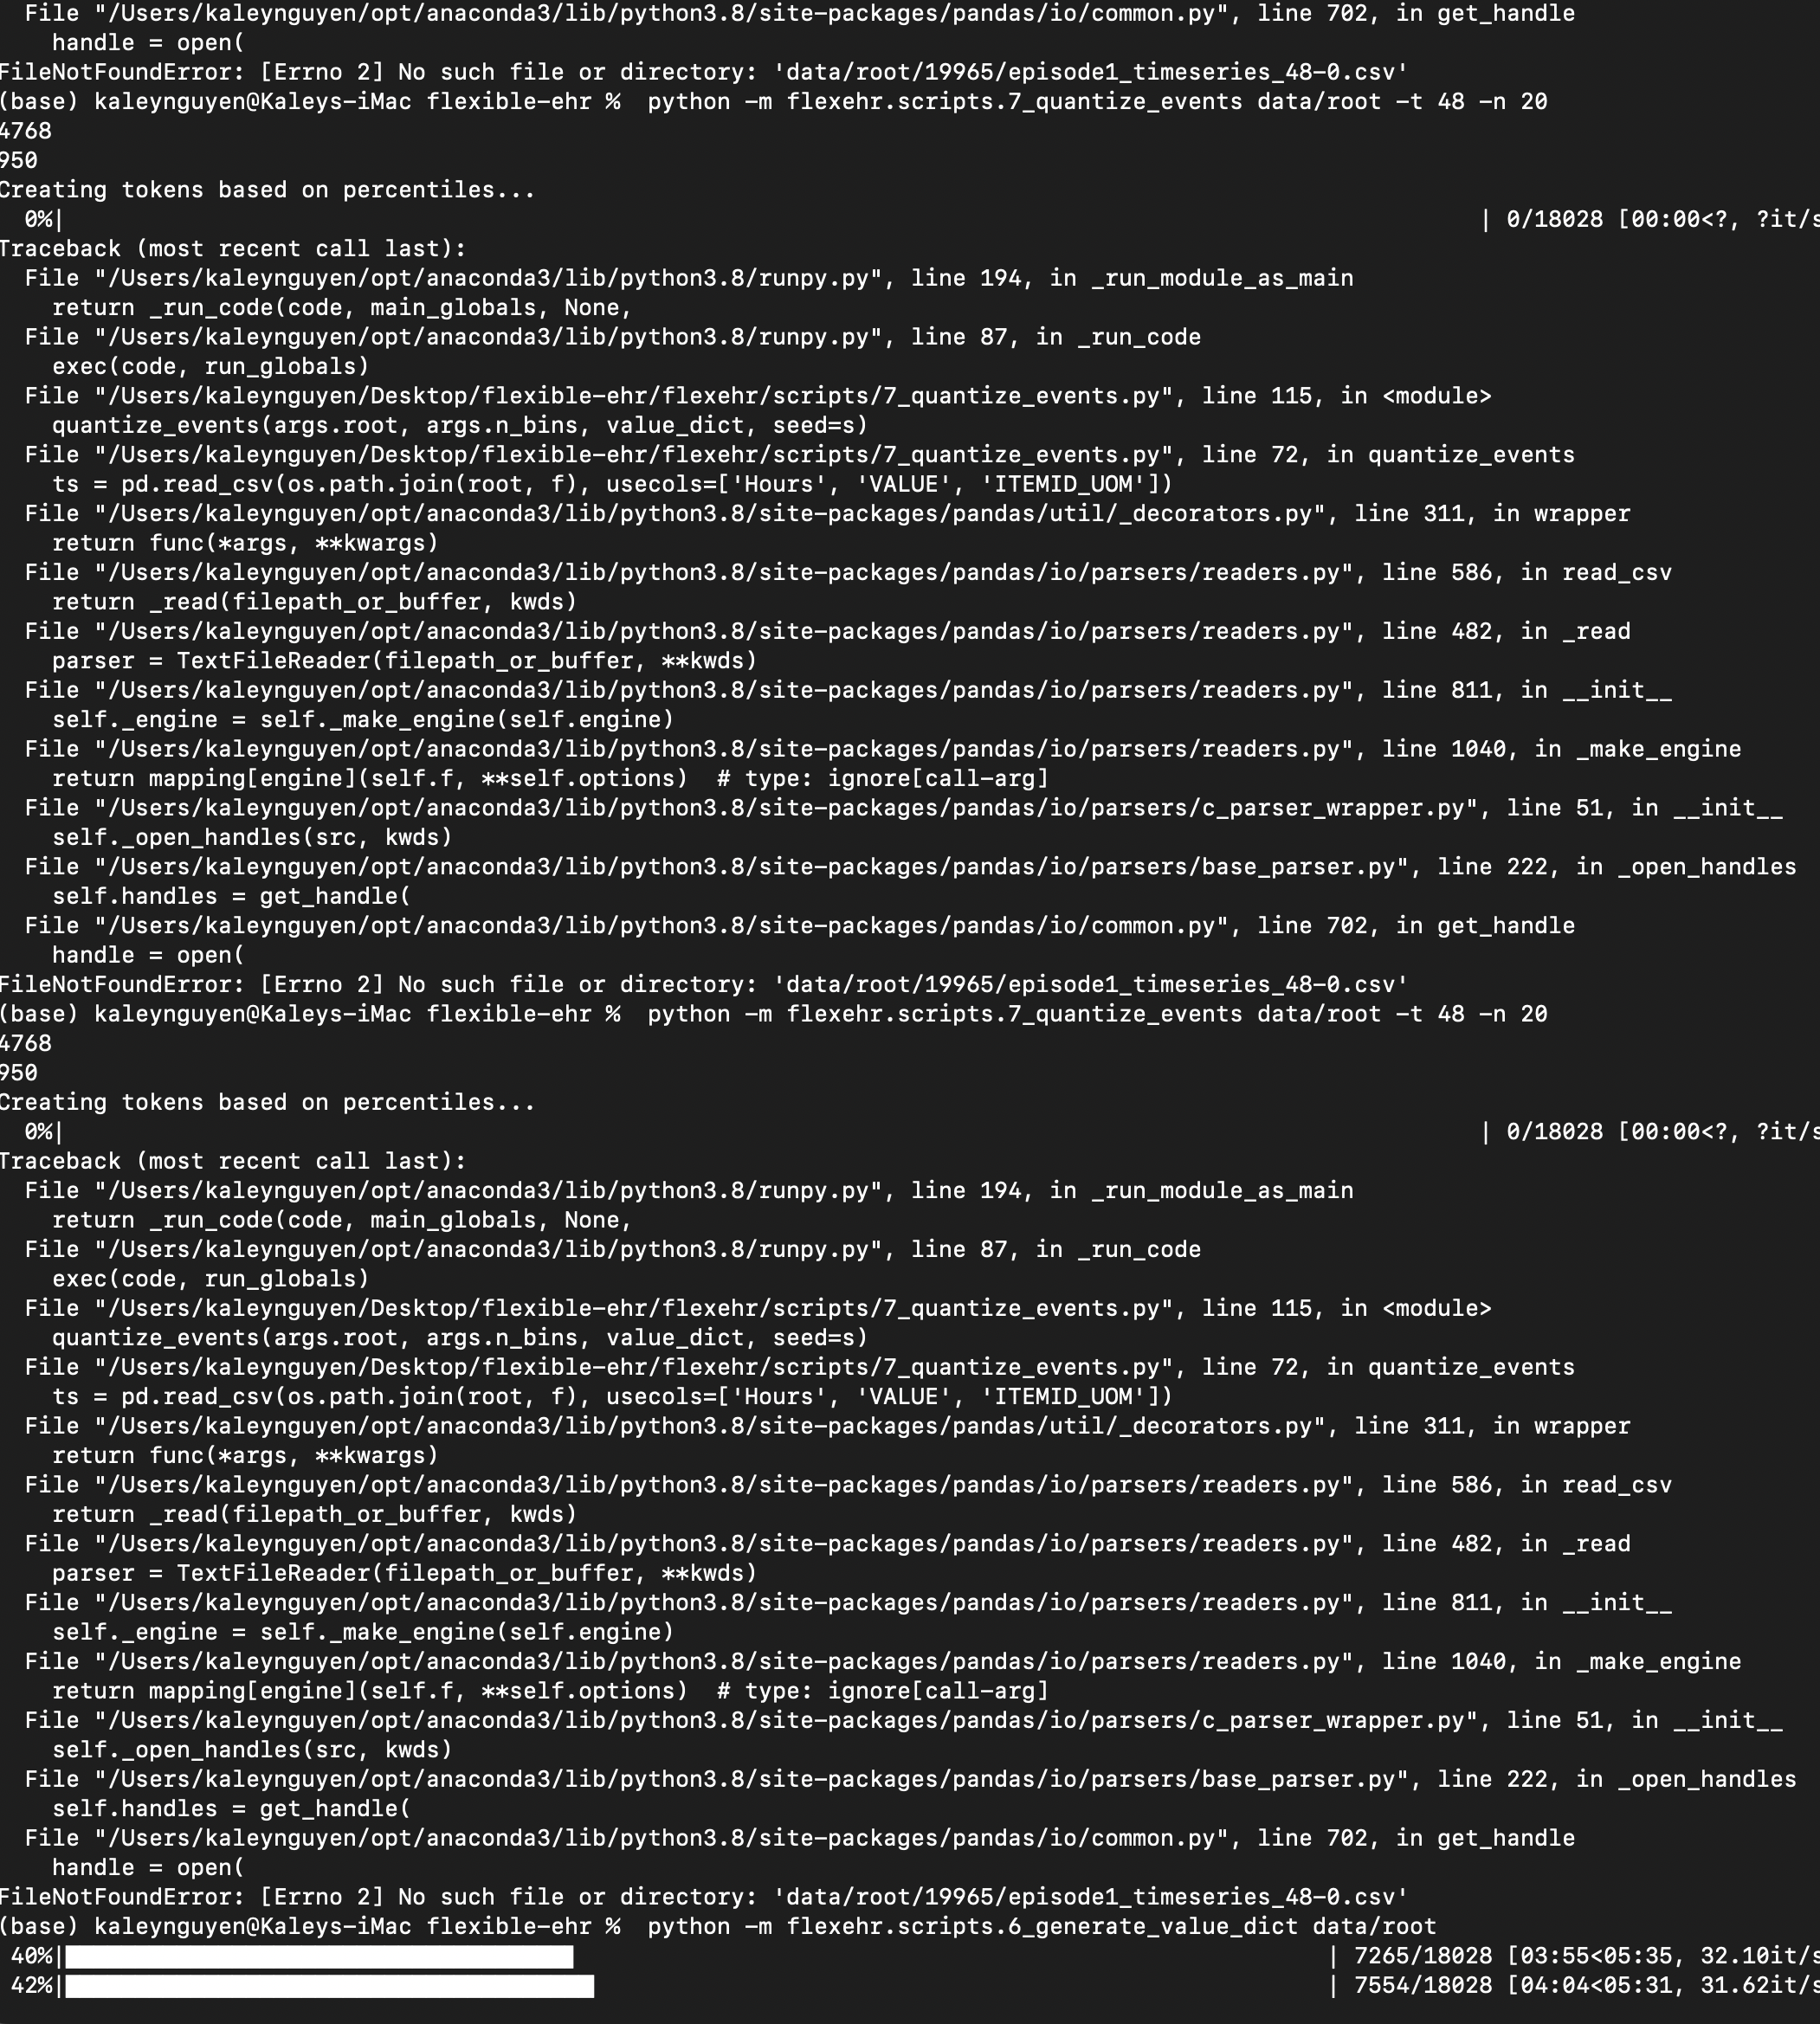
\includegraphics[scale=0.16]{acl-ijcnlp2021-templates/image/cleaning.png}

\subsection{Result 2}
I tried to incorporate a new sampling strategy and a new loss function onto a PyHealth model but I failed to do so. I would need additional help from the TA so I can know what to do in the final report.  


\bibliographystyle{acl_natbib}
\bibliography{acl2021}

%\appendix



\end{document}
